% ===========================================
% Template for ICMC 2015 (version2)
% adapted from earlier LaTeX paper templates for the ICMC, SMC, etc...
% ===========================================

\documentclass{article}
\usepackage{icmc2015template}
\usepackage{times}
\usepackage{ifpdf}
\usepackage{soul}
\usepackage[english]{babel}
\usepackage{cite}
\usepackage{colortbl}
\usepackage{microtype}
\usepackage{units}
\usepackage{paralist}
\usepackage{float}
\restylefloat{table}
\usepackage{caption}

%%%%%%%%%%%%%%%%%%%%%%%% Some useful packages %%%%%%%%%%%%%%%%%%%%%%%%%%%%%%%
%%%%%%%%%%%%%%%%%%%%%%%% See related documentation %%%%%%%%%%%%%%%%%%%%%%%%%%
%\usepackage{amsmath} % popular packages from Am. Math. Soc. Please use the 
%\usepackage{amssymb} % related math environments (split, subequation, cases,
%\usepackage{amsfonts}% multline, etc.)
%\usepackage{bm}      % Bold Math package, defines the command \bf{}
%\usepackage{paralist}% extended list environments
%%subfig.sty is the modern replacement for subfigure.sty. However, subfig.sty 
%%requires and automatically loads caption.sty which overrides class handling 
%%of captions. To prevent this problem, preload caption.sty with caption=false 
%\usepackage[caption=false]{caption}
%\usepackage[font=footnotesize]{subfig}

% ====================================================
% ================ Define title and author names here ===============
% ====================================================
%user defined variables
\def\papertitle{Genre-specific Key Profiles}
\def\firstauthor{Cian O'Brien}
\def\secondauthor{Alexander Lerch}
\def\thirdauthor{Third Author}
\def\fourthauthor{Fourth Author}
\def\fifthauthor{Fifth Author}
\def\sixthauthor{Sixth Author}

% adds the automatic
% Saves a lot of ouptut space in PDF... after conversion with the distiller
% Delete if you cannot get PS fonts working on your system.

% pdf-tex settings: detect automatically if run by latex or pdflatex
\newif\ifpdf
\ifx\pdfoutput\relax
\else
   \ifcase\pdfoutput
      \pdffalse
   \else
      \pdftrue
\fi

\ifpdf % compiling with pdflatex
  \usepackage[pdftex,
    pdftitle={\papertitle},
    pdfauthor={\firstauthor, \secondauthor, \thirdauthor},
    bookmarksnumbered, % use section numbers with bookmarks
    pdfstartview=XYZ % start with zoom=100% instead of full screen; 
                     % especially useful if working with a big screen :-)
   ]{hyperref}
  %\pdfcompresslevel=9

  \usepackage[pdftex]{graphicx}
  % declare the path(s) where your graphic files are and their extensions so 
  %you won't have to specify these with every instance of \includegraphics
  \graphicspath{{./figures/}}
  \DeclareGraphicsExtensions{.pdf,.jpeg,.png}

  \usepackage[figure,table]{hypcap}

\else % compiling with latex
  \usepackage[dvips,
    bookmarksnumbered, % use section numbers with bookmarks
    pdfstartview=XYZ % start with zoom=100% instead of full screen
  ]{hyperref}  % hyperrefs are active in the pdf file after conversion

  \usepackage[dvips]{epsfig,graphicx}
  % declare the path(s) where your graphic files are and their extensions so 
  %you won't have to specify these with every instance of \includegraphics
  \graphicspath{{./figures/}}
  \DeclareGraphicsExtensions{.eps}

  \usepackage[figure,table]{hypcap}
\fi

%setup the hyperref package - make the links black without a surrounding frame
\hypersetup{
    colorlinks,%
    citecolor=black,%
    filecolor=black,%
    linkcolor=black,%
    urlcolor=black
}


% ====================================================
% ================ Title and author info starts here ===============
% ====================================================
% Title.
% ------
\title{\papertitle}

% Authors
% Please note that submissions are anonymous, therefore 
% authors' names should not be VISIBLE in your paper submission.
% They should only be included in the camera-ready version of accepted papers.
% uncomment and use the appropriate section (1, 2 or 3 authors)
%
% Single address
% To use with only one author or several with the same address
% ---------------
\oneauthor
   {\firstauthor \qquad \secondauthor} {Center for Music Technology \\ Georgia Institute of Technology \\ %
     {\tt \href{mailto:\@unt.edu}{\{cobrien30, alexander.lerch\}@gatech.edu}}}

%Two addresses
% the default spacing is 1.5in, but this can be reduced to 0.5in or less, if needed
%--------------
% \twoauthors
%   {1.5in}
%   {\firstauthor} {Affiliation1 \\  %
%     {\tt \href{mailto:author1@unt.edu}{author1@unt.edu}}}
%   {\secondauthor} {Affiliation2 \\  %
%     {\tt \href{mailto:author2@unt.edu}{author2@unt.edu}}}

% Three addresses
% the default spacing is 0.5in, but this can be reduced to 0.3in or less, if needed
% --------------
% \threeauthors
%   {0.5in}
%   {\firstauthor} {Affiliation1 \\ %
%     {\tt \href{mailto:author1@unt.edu}{author1@unt.edu}}}
%   {\secondauthor} {Affiliation2 \\ %
%     {\tt \href{mailto:author2@unt.edu}{author2@unt.edu}}}
%   {\thirdauthor} { Affiliation3 \\ %
%     {\tt \href{mailto:author3@unt.edu}{author3@unt.edu}}}

% Four addresses
% the default spacing is 1.5in, but this can be reduced to 0.5in or less, if needed
% --------------
% \fourauthors
%   {1.5in}
%   {\firstauthor} {Affiliation1 \\ %
%     {\tt \href{mailto:author1@unt.edu}{author1@unt.edu}}}
%   {\secondauthor} {Affiliation2 \\ %
%     {\tt \href{mailto:author2@unt.edu}{author2@unt.edu}}}
%   {\thirdauthor} { Affiliation3 \\ %
%     {\tt \href{mailto:author3@unt.edu}{author3@unt.edu}}}
%   {\fourthauthor} { Affiliation4 \\ %
%     {\tt \href{mailto:author4@unt.edu}{author4@unt.edu}}}

% Five addresses
% the default spacing is 0.5in, but this can be reduced to 0.3in or less, if needed
% --------------
% \fiveauthors
%   {0.5in}
%   {\firstauthor} {Affiliation1 \\ %
%     {\tt \href{mailto:author1@unt.edu}{author1@unt.edu}}}
%   {\secondauthor} {Affiliation2 \\ %
%     {\tt \href{mailto:author2@unt.edu}{author2@unt.edu}}}
%   {\thirdauthor} { Affiliation3 \\ %
%     {\tt \href{mailto:author3@unt.edu}{author3@unt.edu}}}
%   {\fourthauthor} { Affiliation4 \\ %
%     {\tt \href{mailto:author4@unt.edu}{author4@unt.edu}}}
%   {\fifthauthor} { Affiliation5 \\ %
%     {\tt \href{mailto:author5@unt.edu}{author5@unt.edu}}}

% Six addresses
% the default spacing is 0.5in, but this can be reduced to 0.3in or less, if needed
% --------------
% \sixauthors
%   {0.5in}
%   {\firstauthor} {Affiliation1 \\ %
%     {\tt \href{mailto:author1@unt.edu}{author1@unt.edu}}}
%   {\secondauthor} {Affiliation2 \\ %
%     {\tt \href{mailto:author2@unt.edu}{author2@unt.edu}}}
%   {\thirdauthor} { Affiliation3 \\ %
%     {\tt \href{mailto:author3@unt.edu}{author3@unt.edu}}}
%   {\fourthauthor} { Affiliation4 \\ %
%     {\tt \href{mailto:author4@unt.edu}{author4@unt.edu}}}
%   {\fifthauthor} { Affiliation5 \\ %
%     {\tt \href{mailto:author5@unt.edu}{author5@unt.edu}}}
%   {\sixthauthor} { Affiliation6 \\ %
%     {\tt \href{mailto:author6@unt.edu}{author6@unt.edu}}}


% ====================================================
% =============== The document content starts here ===============
% ====================================================
\begin{document}
%
\capstartfalse
\maketitle
\capstarttrue
%
\begin{abstract}
The most common approaches to the automatic recognition
of musical key are template-based, i.e., an extracted pitch
chroma vector is compared to a template key profile in order
to identify the most similar key. General as well as domainspecific templates have been used in the past, but to the authors’ best knowledge there has been no study that evaluated
genre-specific key profiles extracted from the audio signal. We
investigate the pitch chroma distributions for 9 different genres, their distances, and the degree to which these genres can
be identified using these distributions when utilizing different
strategies for achieving key-invariance.
\end{abstract}
%

\section{Introduction}\label{sec:introduction}
The pitch chroma is a compact and robust representation of
the tonal content of an audio signal. Automatic key detection
systems commonly use the average pitch chroma of a music
file in order to detect the musical key by comparing the extracted pitch chroma to a template key profile. In the literature,
different strategies for deriving these templates have been proposed, such as based on human tonality perception \cite{krumhansl_cognitive_1990}, using
diatonic models \cite{izmirli_template_2005}, extraction from MIDI data \cite{temperley_pitch-class_2008}, and extraction from audio data \cite{van_de_par_musical_2006}. Here we analyze the distributions
of (pitch chroma based) key profiles extracted from different
musical genres. The similarity of genre-specific key profiles
is measured directly by computing inter-genre distances in
Sect. 4 and indirectly by applying an SVM classifier for testing genre separability through key profiles (Sect. 5). The goal
of this work is to investigate (i) how pitch chroma are distributed within each genre and (ii) the extent to which musical
genres can be distinguished using only the tonal information
contained in their pitch chroma profiles.

\section{Data set}\label{sec:dataset}
The data set used was the GTZAN collection.\footnote{\url{http://marsyas.info/downloads/datasets.html}}
While this set
is old and has obvious disadvantages \cite{sturm_analysis_2012}, it is a well-known, widely-used, and easily available set for genre classification tasks. It consists of $1000$ song excerpts divided into ten genres: Blues (\textit{B}), Classical  (\textit{Cl}), Disco (\textit{D}), Reggae (\textit{Rg}), Pop (\textit{P}), Metal (\textit{M}), Rock (\textit{R}), Jazz (\textit{J}), Country (\textit{C}) and Hip Hop (\textit{H}). 
Key annotations for the tracks are publicly available.\footnote{\url{https://github.com/alexanderlerch/data_set}}%github.com/alexanderlerch/data_set}}
 %Figure~\ref{tab:NumberOfAnnotatedDataSetEntries} gives an overview of the number of annotated files and their mode. The number of annotated files therefore reflects the number of unambiguously identifyable keys.
%For example, none of the excerpts from the Classical genre are annotated. 
%Tracks for which the key could not be unambigiously identified were excluded, which includeed all examples in the Classical genre. ttfgds fsd fsd fs fsd fsd sdf  sdf dsf sdf sdf sd sdf dsf ds fs sdfs dfsd fds  sdf dsf sd fdsf 
Tracks for which the key could not be unambigiously identified were excluded. The number of annotated files therefore reflects the number of unambiguously identifyable keys.
For example, none of the excerpts from the Classical genre are annotated. 

Figure \ref{fig:KeyDistributionPerGenre} gives a more detailed visualization of the key distribution per genre with the tonics sorted with respect to the circle of fifths and major modes (left) separated from minor modes (right). 
%The distribution of keys in each genre proved unsurprising.
The relation of major vs.\ minor modes is very skewed for blues and metal (predominantly minor) as well as country (predominantly major); the genres disco, pop, reggae, and rock have a more balanced distribution between modes. Jazz tracks tend to be clustered around flat keys which are favored by trumpet and saxophone players. The keys for country cluster around C-Maj with a tendency to sharp keys. The majority of metal tracks are in either a minor or e minor, keys well-suited to the electric guitar and bass (corresponding to the two lowest open strings).

%Pieces from the blues are mostly in the keys of G, E and B-flat. 

%It is worth noting that Li and Chan presented another set of key annotations for the GTZAN data set \cite{li_genre_2011}. An examination of the two independent annotations reveals some disagreements between the two annotations: overall, about $85$ percent of the data is labeled identically. 
%%ICH VERSTEHE DIE ZAHLEN HIER NICHT: 67 + 119 IST DOCH MEHR ALS 15\%??%
%Of the differences where there was disagreement on whether one key was clearly identifiable or not, the majority were found in the Blues genre with 67 out 127 total disagreements of this type. If we consider only examples where both analyses agreed a modulation had \textit{not} occurred, there was a total of 119 disagreements. The most common differences were: major/relative-minor confusion (38), tonic/fifth confusion (35) and major/minor confusion (13).
%\begin{itemize}
    %\item   blues: $98$ vs.\ $31$ (Li) annotated tracks
    %\item   disco: $21$ differences between the two data sets
%\end{itemize}
%The genre country showed only $1$ difference. 

\section{Feature extraction}\label{sec:pitch_chroma}

%\subsection{Pitch chroma}\label{subsec:pc_extract}
The \textit{pitch chroma} is a commonly used feature in the field of MIR  because it is a compact, robust, and mostly timbre-independent representation of the pitch content  \cite{muller_information_2007}. It is a $12$-dimensional histogram-like octave-independent vector showing the ``strength'' of the $12$ semitone classes (C, C\#, D, ..., B) and is computed by converting the spectrum to semi-tone bands and summing the energy of all bands with the distance of an octave \cite{fujishima_realtime_1999}. 
The pitch chroma is extracted at a sample rate of \unit[10]{kHz} over a range of three octaves, starting from C at \unit[130.8]{Hz}. The FFT block size is 8192, the hop size is 4096.
The overall pitch chroma per file is a single 12-dimensional vector that is computed by taking the median of all pitch chromas per block. 

 %Each track in the labeled collection was down-sampled to 10kHz and pitch chroma vectors were extracted block-wise over a three octave range, starting from C = 130.8 Hz. Pitch chroma were then normalized using the 1-norm:                     
	 %equation?
%After extracting pitch chroma for each block we can also average them over whole tracks to obtain an “averaged pitch chroma” for each track, sometimes called a Pitch Histogram [**ref]. After averaging using the median for each chroma-bin each song is then represented by a single 12-dimensional chroma vector.

\begin{figure}[tb]\label{tab:NumberOfAnnotatedDataSetEntries}
    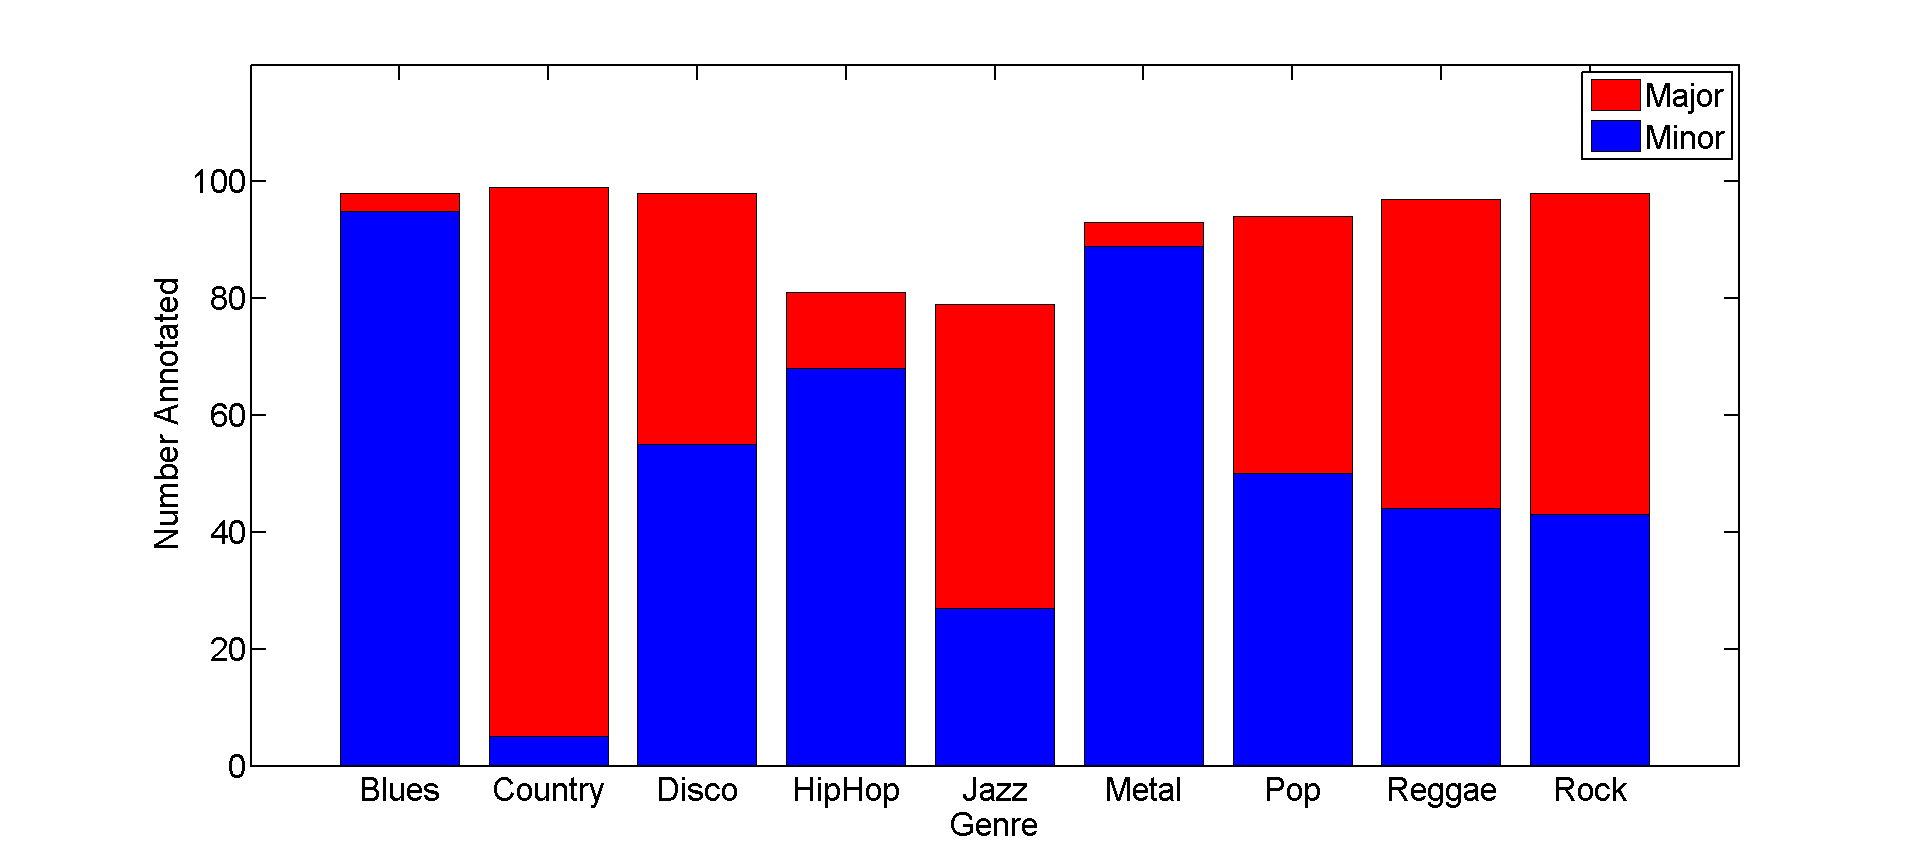
\includegraphics[scale=.2]{graph/annotated}
	\caption{Per genre major/minor distributions and number of annotated files}
	\label{fig:confPC+MFCC}
\end{figure}


%\subsection{Key profiles}\label{sec:featureset}
The term \textit{key profile} is used for the overall, tonic independent pitch chroma per file. We assume that the key profiles of songs within one genre that have the same mode (major or minor) should be similar, but shifted circularly to the songs' tonic. Under this assumption, each overall pitch chroma can be ``converted'' to a key-profile by applying a circular shift. In other words, the key profile is the tonic independent pitch distribution (e.g., the pitch chroma of a song in A-Maj or a-min is circularly shifted by $9$ indices to the left so that the bin of pitch class A lands on the first index).

%A problem with using a pitch chroma approach is that the overall tonality of each song may dominate any between-genre differences; because the distribution of major and minor keys are not the same for each genre, songs might be classified according to their key using this method. For example pitch chroma extracted from minor tracks would be classified as Metal, since the averaged pitch chroma for Metal would be obtained by averaging pitch chroma extracted from predominantly minor tracks. This is an inherent problem in using pitch chroma as op-posed to more often used timbral features like MFCCs and in order to account for this we processed major and minor tracks separately. Another consideration revealed in the analysis of the data set is that the the key-labels are not uniformly distributed within each key. For example the majority of songs in the keys of A and E-minor are in the Rock and Metal genres. 

\section{Key Profile Analysis}\label{keyprof}
%In order to generate the key profiles for this overall analysis, we used the the KP1 key profiles.
%\subsection{Overall key profiles}
Figure \ref{fig:OverallKeyProfiles} shows the overall key profiles in a box plot in comparison with known profiles from the literature. 
While Krum\-hansl's ``Probe Tone Ratings'' \cite{krumhansl_cognitive_1990} are not exactly a key profile (derived from listening experiments on tonality), they correlate well with key profiles (compare \cite{izmirli_template_2005}). 
Temperley's key profiles are extracted from symbolic data  rather than from audio \cite{temperley_bayesian_2004,temperley_pitch-class_2008}.
\begin{figure*}[htb]\setcounter{figure}{2}
\centering
    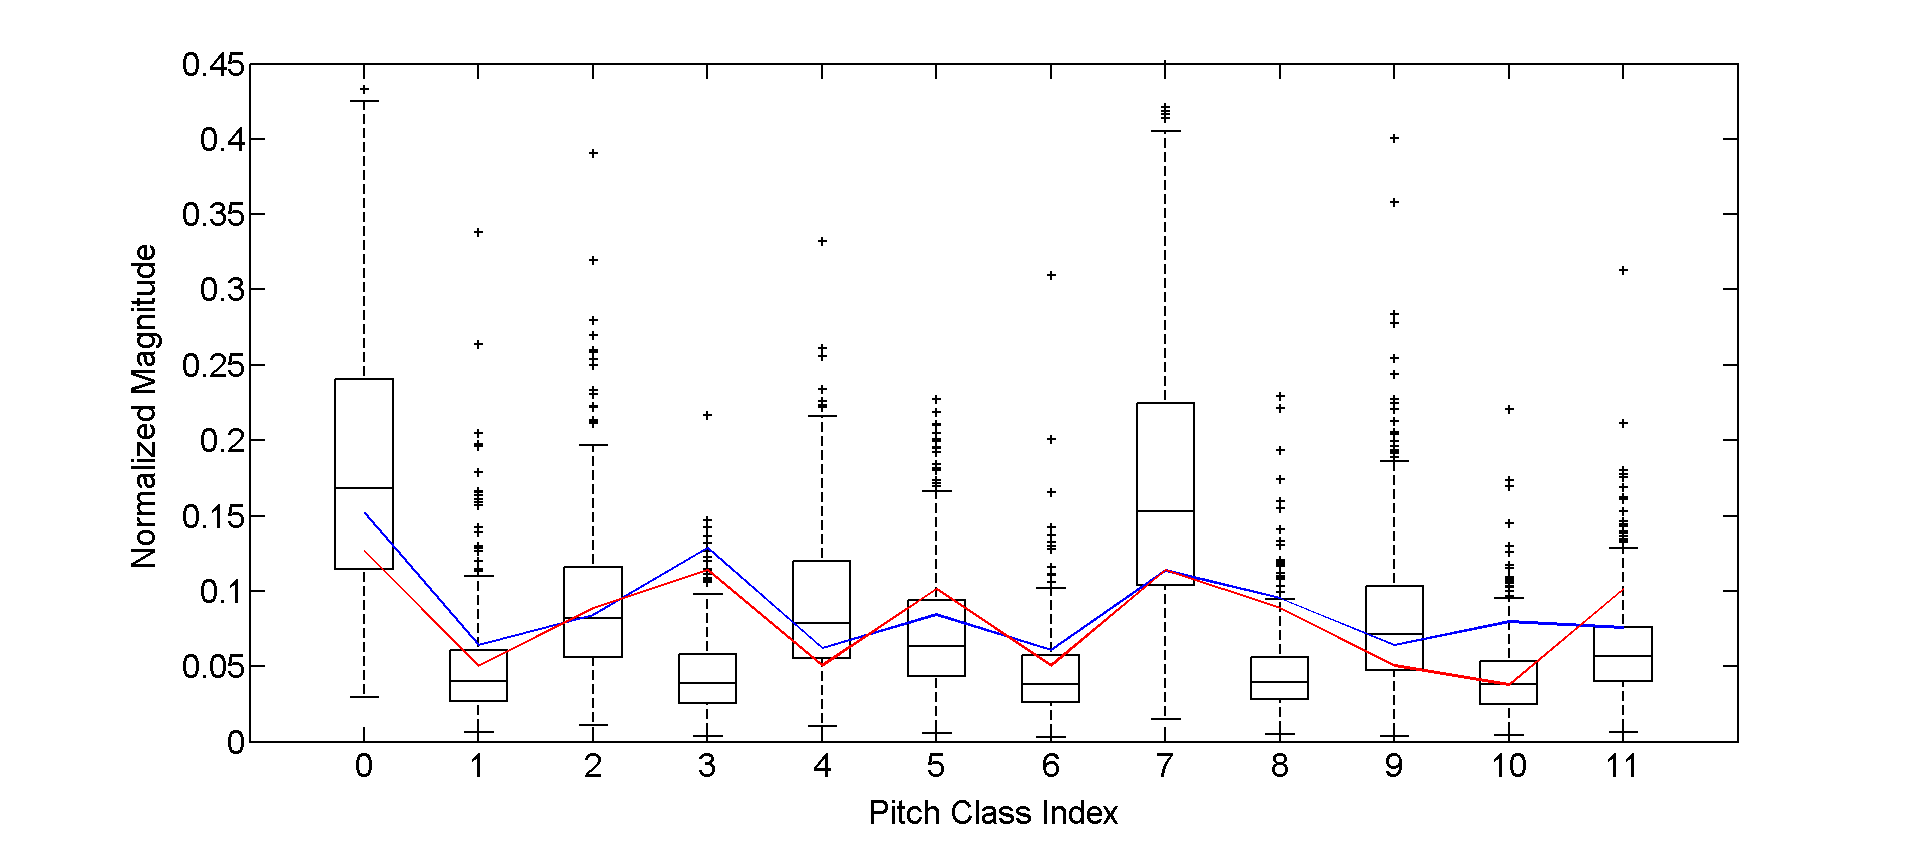
\includegraphics[scale=.2]{graph/allMajChroma+Krum+Temp}
    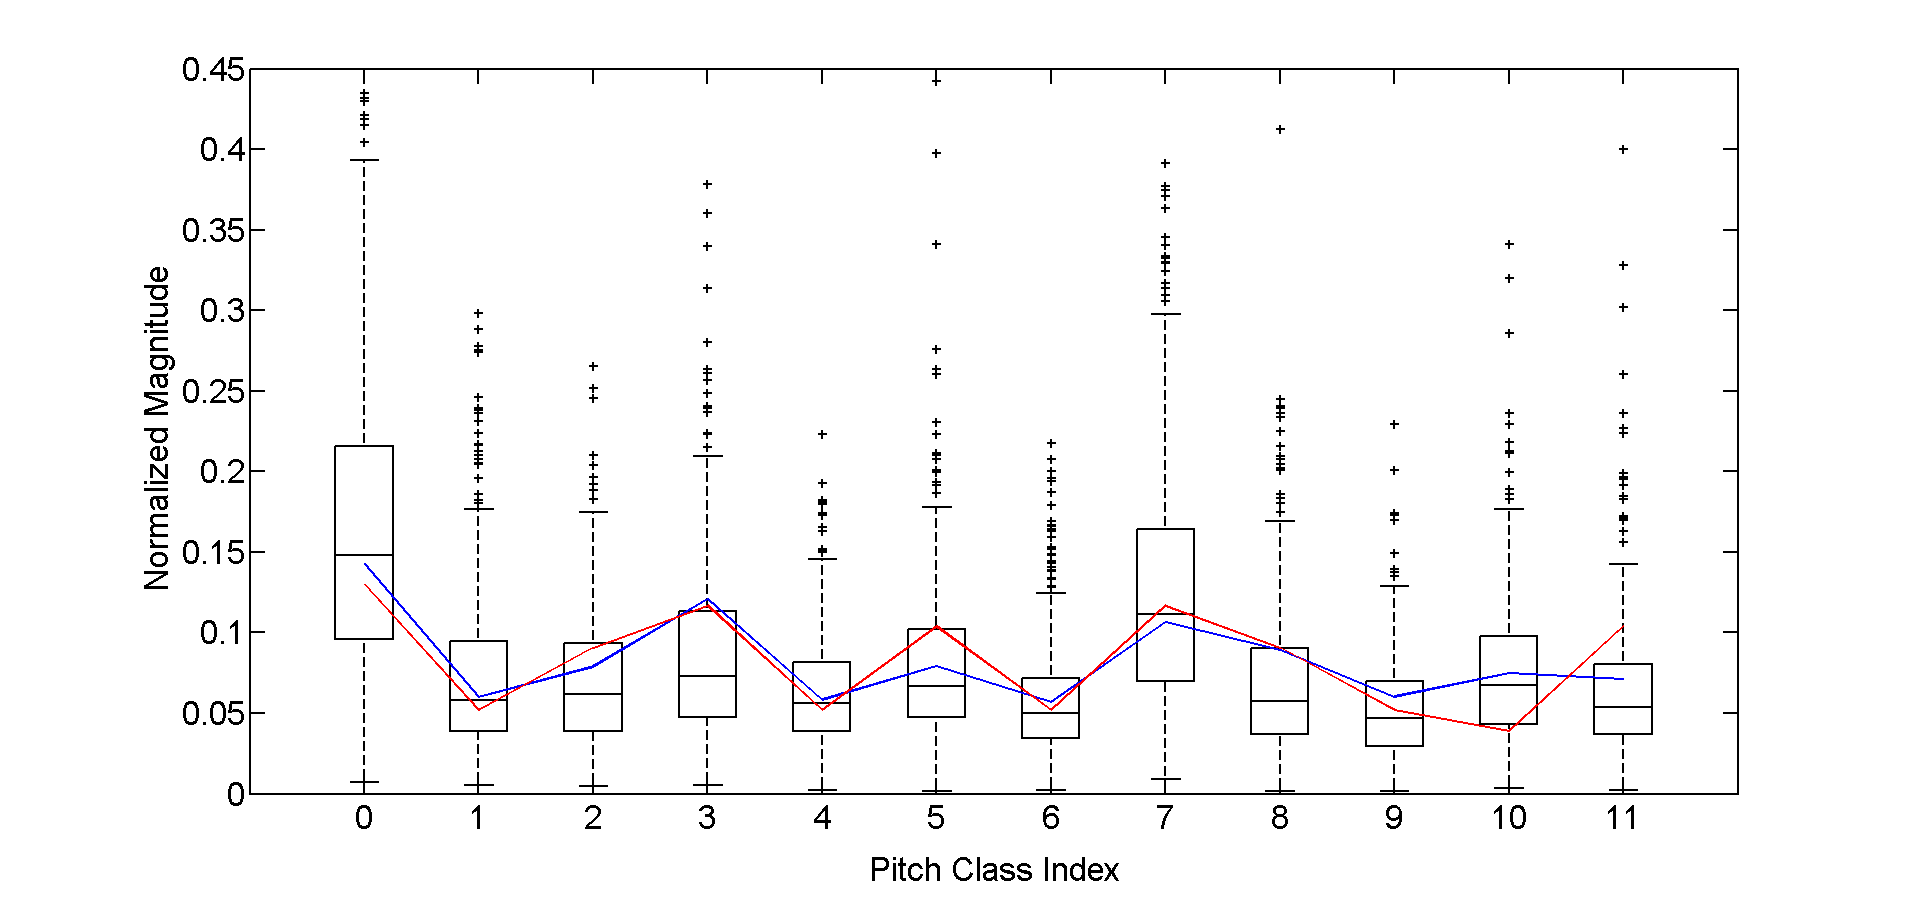
\includegraphics[scale=.2]{graph/allMinChroma+Krum+Temp}
	\caption{Major (left) and minor (right) key profiles for the complete data set, in comparison with two widely-used key profiles (Krumhansl in red and Temperley in blue).}
	\label{fig:OverallKeyProfiles}
\end{figure*}

%\subsection{Genre-specific key profiles}
The key profiles of the six most populated genres are plotted in Fig.~\ref{fig:SpecificKeyProfiles}.
\begin{figure*}[tb]\setcounter{figure}{3}
\centering
    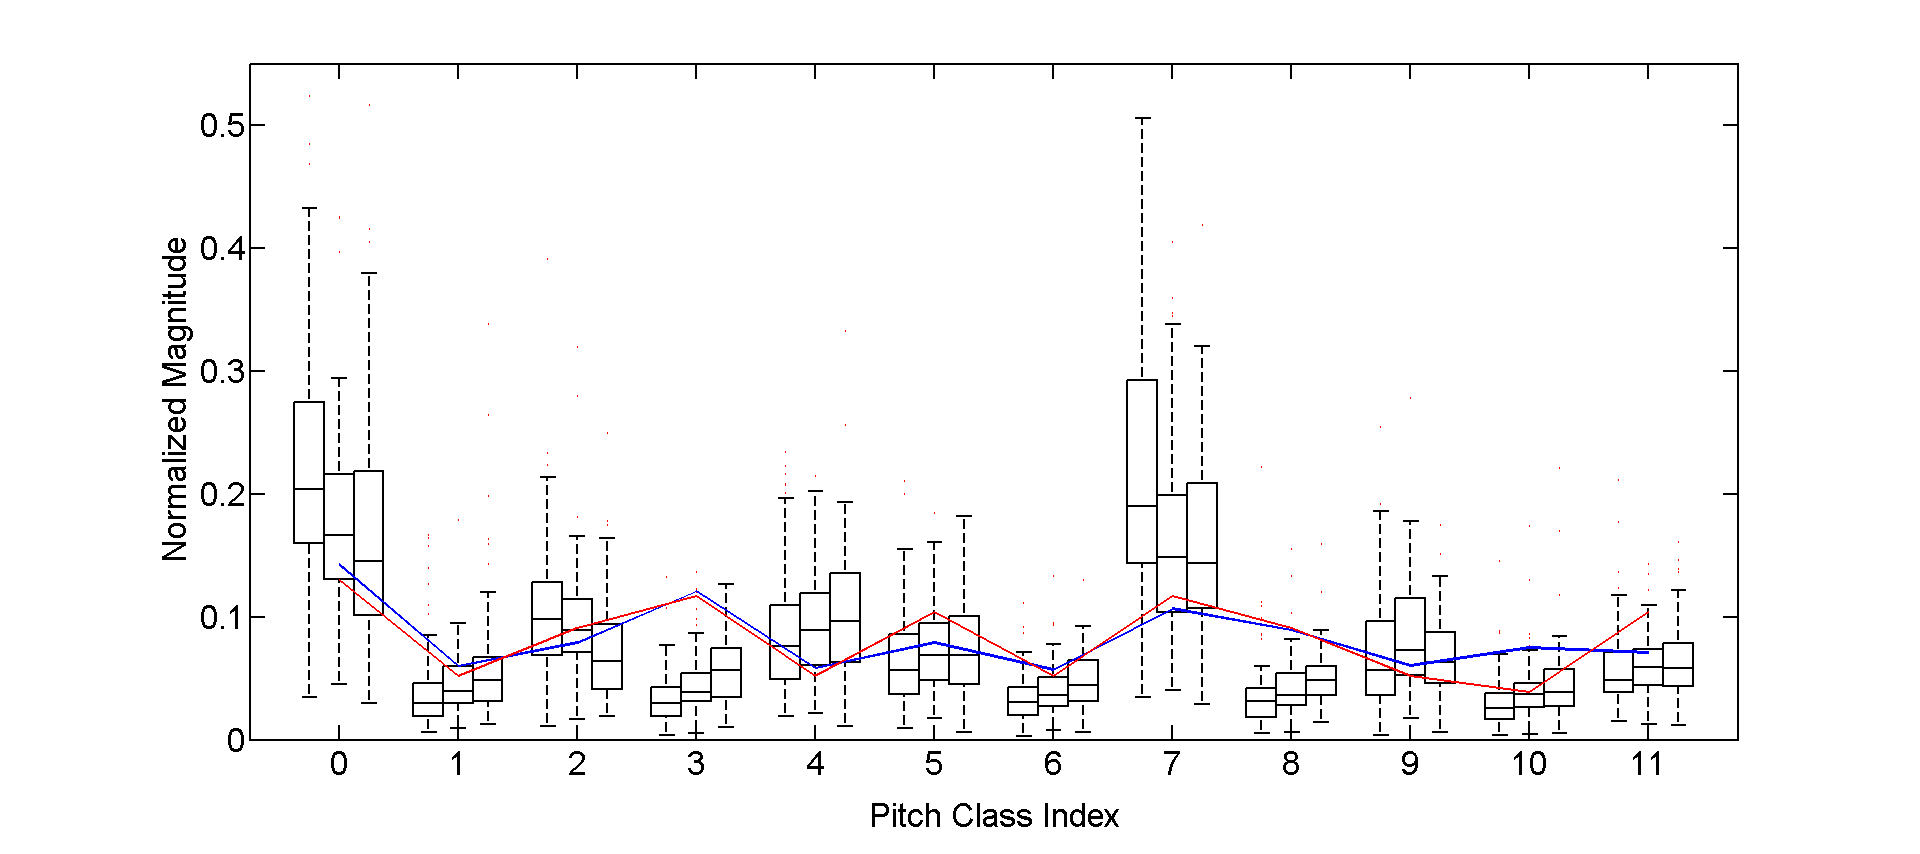
\includegraphics[scale=.2]{graph/boxPlotsMajCPR+Krum+Temp}
    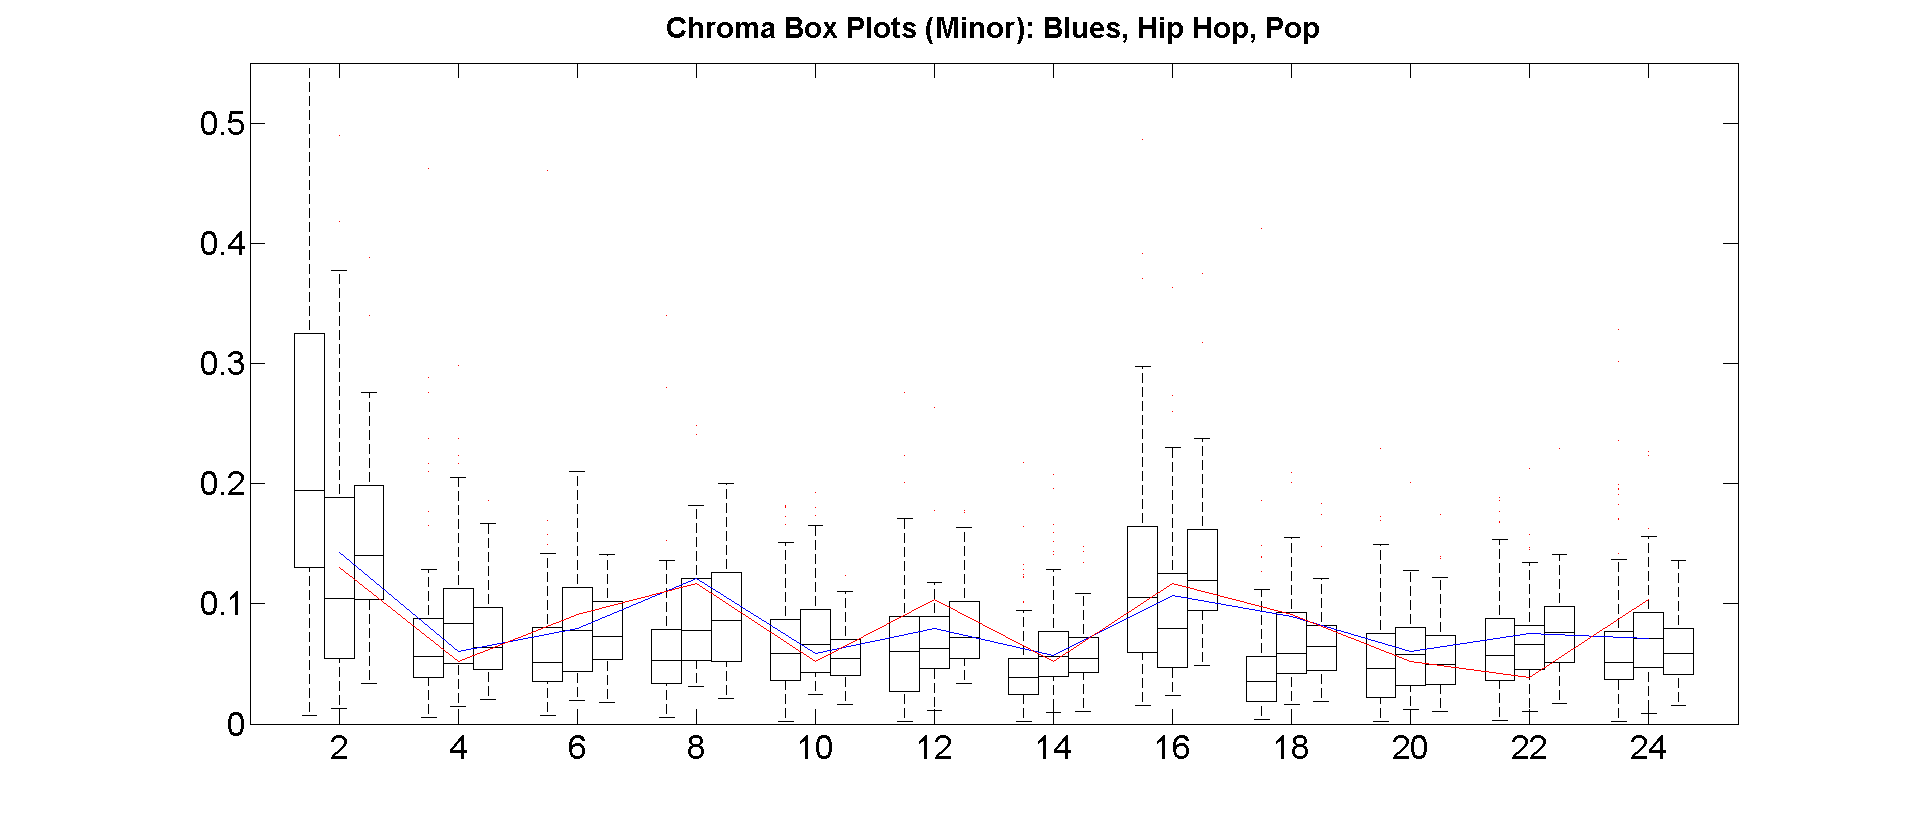
\includegraphics[scale=.2]{graph/boxPlotsMinBHP+Krum+Temp}
    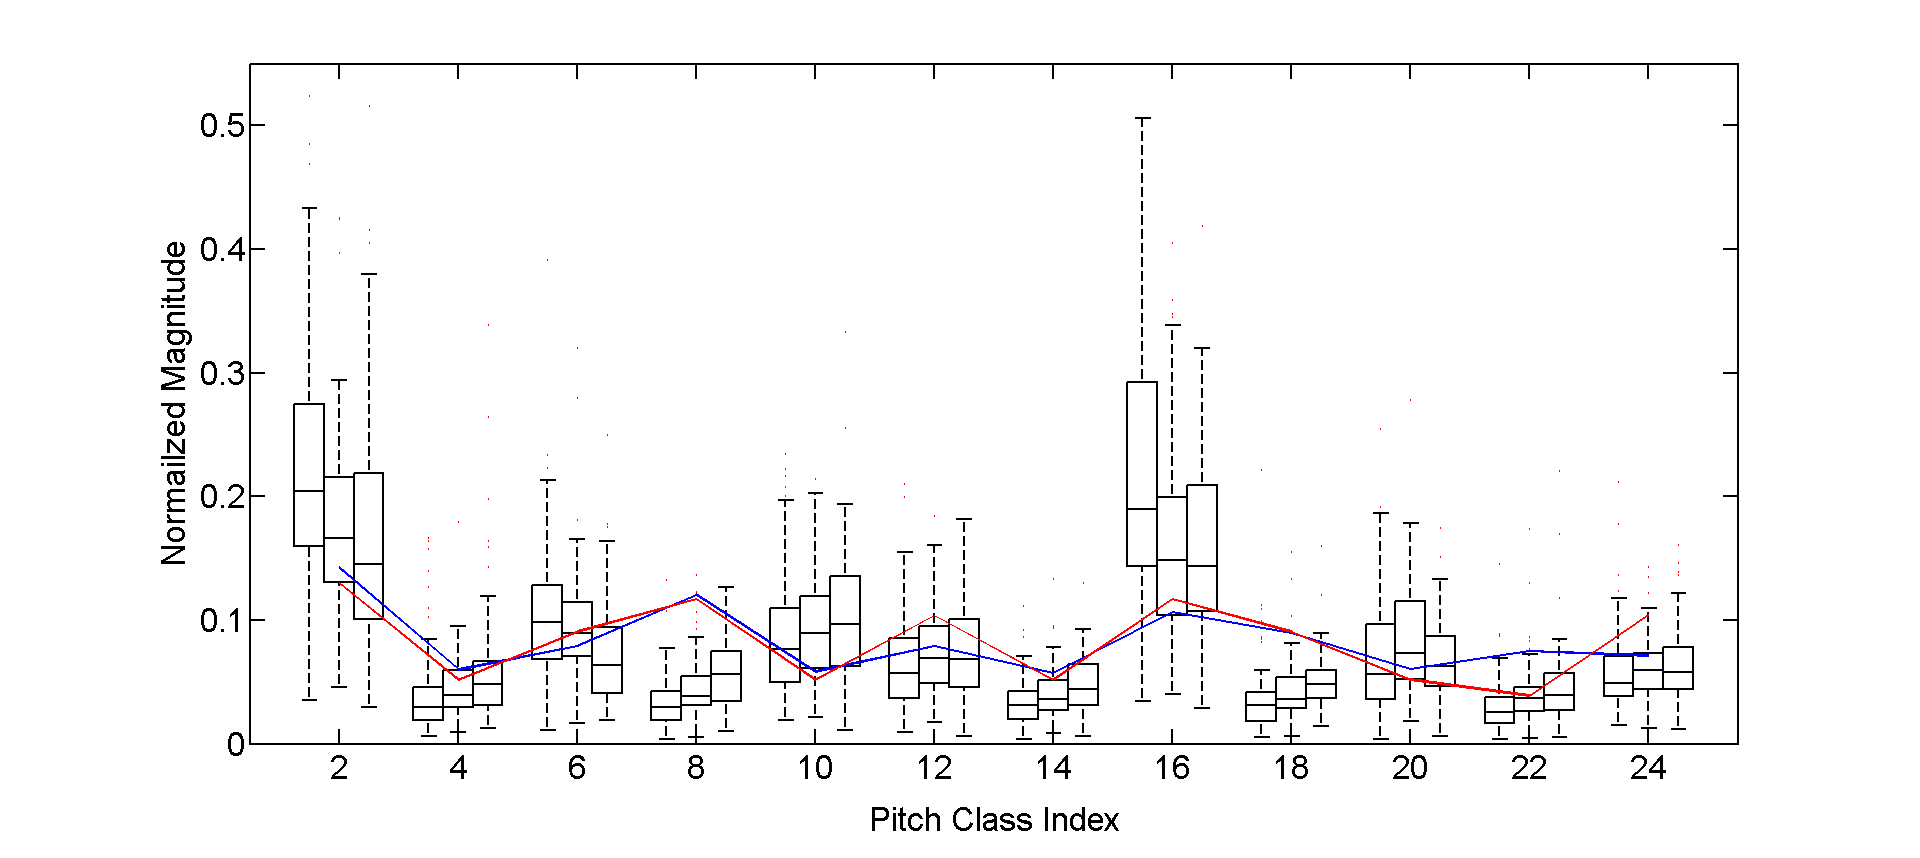
\includegraphics[scale=.2]{graph/boxPlotsMajDJRk+Krum+Temp}
    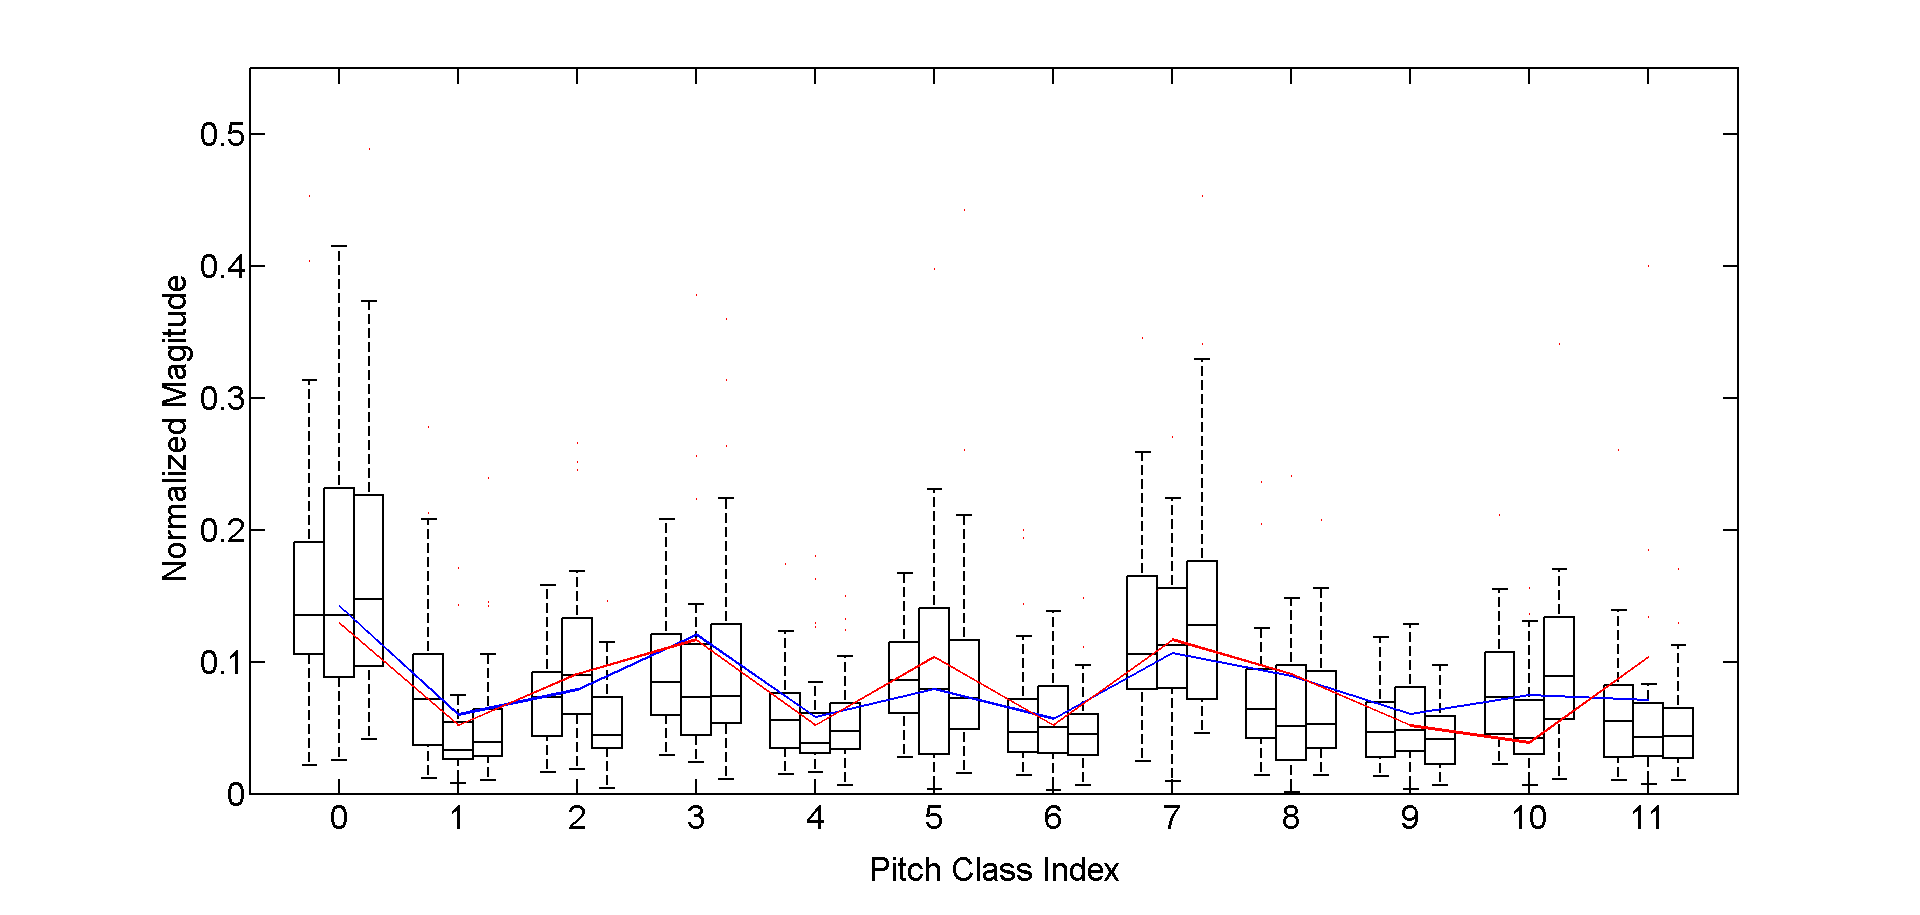
\includegraphics[scale=.2]{graph/boxPlotsMinDMR+Krum+Temp}
	\caption{Major (left) and minor (right) key profiles for the six most populated genres, in comparison with the Krumhansl (red) and Temperley (blue) profiles. Major genres are country, pop, reggae (top left) and disco, jazz and rock (bottom left). Minor genres are blues, hip hop and pop (top right) and disco, metal and reggae (bottom right).}
	\label{fig:SpecificKeyProfiles}
\end{figure*}
The major distribution exhibits mostly a similar pattern with prominent spikes at the tonic and the fifth. The Jazz key profile is one example that is noticeably different: it is rather flat compared to the distributions of other genre's. It is to be expected that Jazz shows a wider range of pitches and harmonies and has thus a more uniformly distributed key profile.

The key profiles for minor have, compared to the major profiles, less distinct minima for non-scale pitches; especially the Blues profile is ---~with the exception of tonic and fifth~--- basically uniformly distributed.

\subsection{Inter-genre distances}
In order to evaluate how distinct genres are with respect to their key profile, distances between all profiles were calculated using the Manhattan distance as shown in Tables~\ref{tab:GenreDistancesMinor} and \ref{tab:GenreDistancesMajor}. Genres for which the number of examples were less than 30 are grayed out. The labels are as introduced above, plus \textit{Kr} for the Krumhansl key profile,  and \textit{Tp} the Temperley profile \cite{temperley_tonal_2007}. The median major/minor profiles over all genres are denoted by \textit{Mdn}.
With respect to major key profile distances, the most similar genres are Rock and Pop while the most mutually distinct genres are Country and Reggae. For minor tracks, Disco and Pop are the most similar while Reggae and Blues are the most distinct.

%To further explore the genre relationships we use Multidimensional Scaling, a method for visualizing information contained in an arbitrary distance matrix  by projecting  the data  into a  space of  smaller  dimension while preserving the between-item distances as well as possible; i.e., the Euclidean distance in the new space will approximate the dissimilarity in the distance matrix. These plots are presented in Fig.~\ref{fig:MDS}. \textbf{Maybe remove this paragraph and the figures to save space?}
%%
%\begin{figure}
    %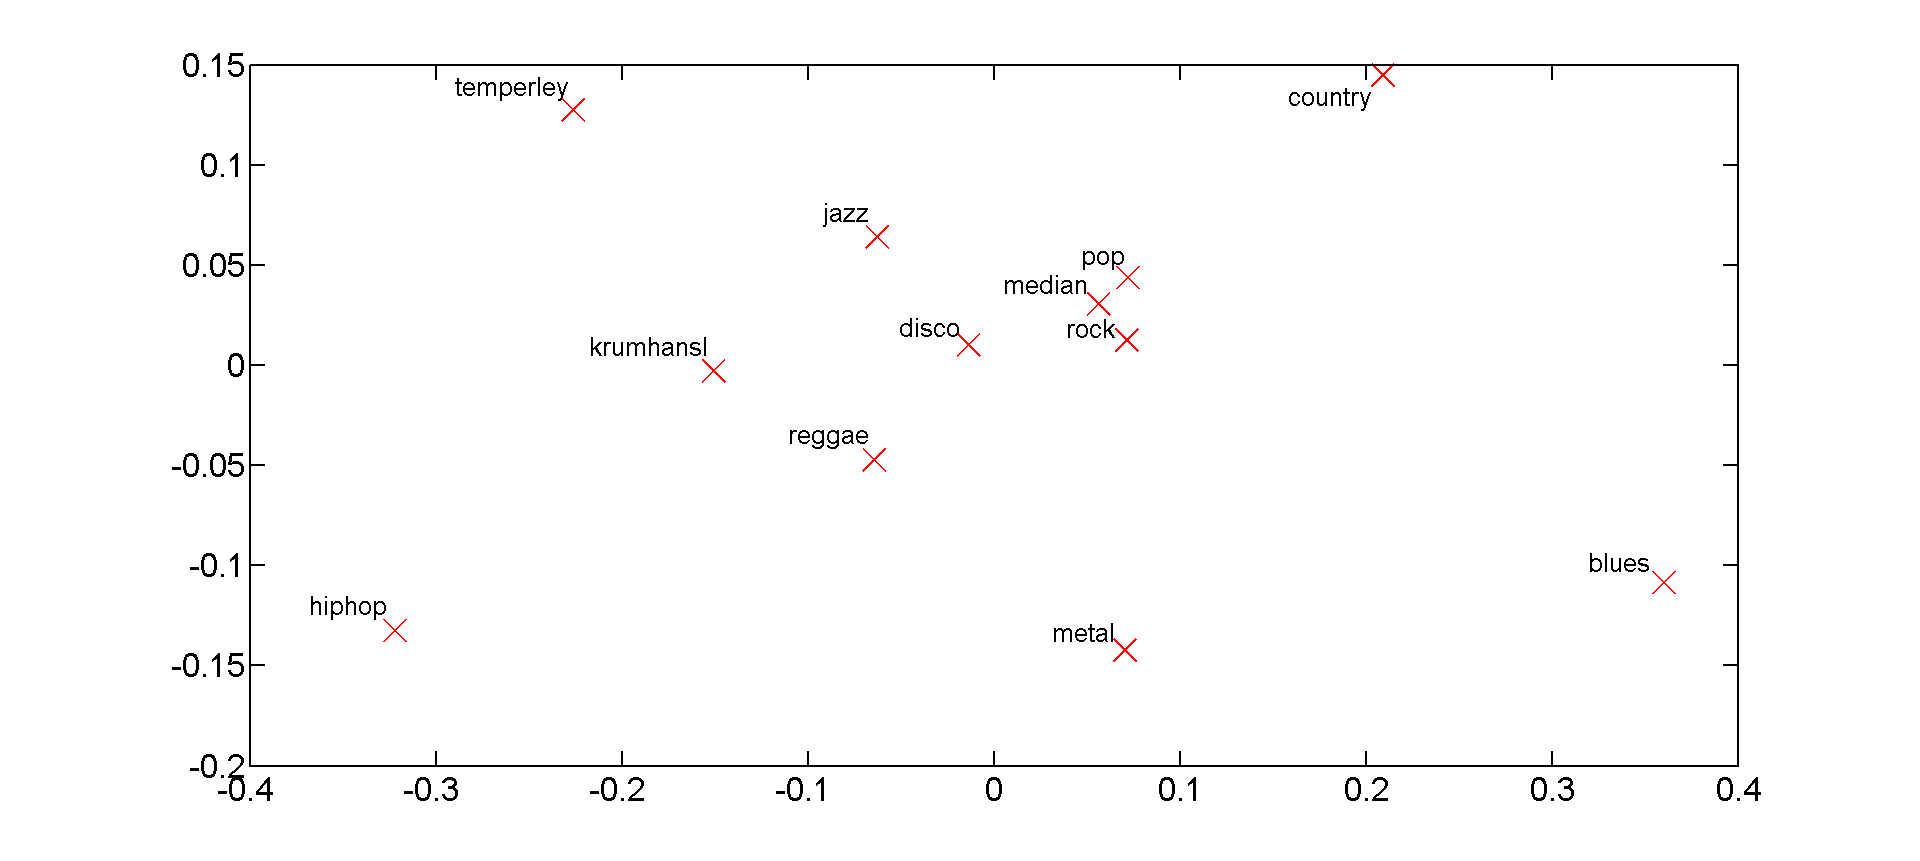
\includegraphics[scale=.2]{graph/MDS_maj_colour}
    %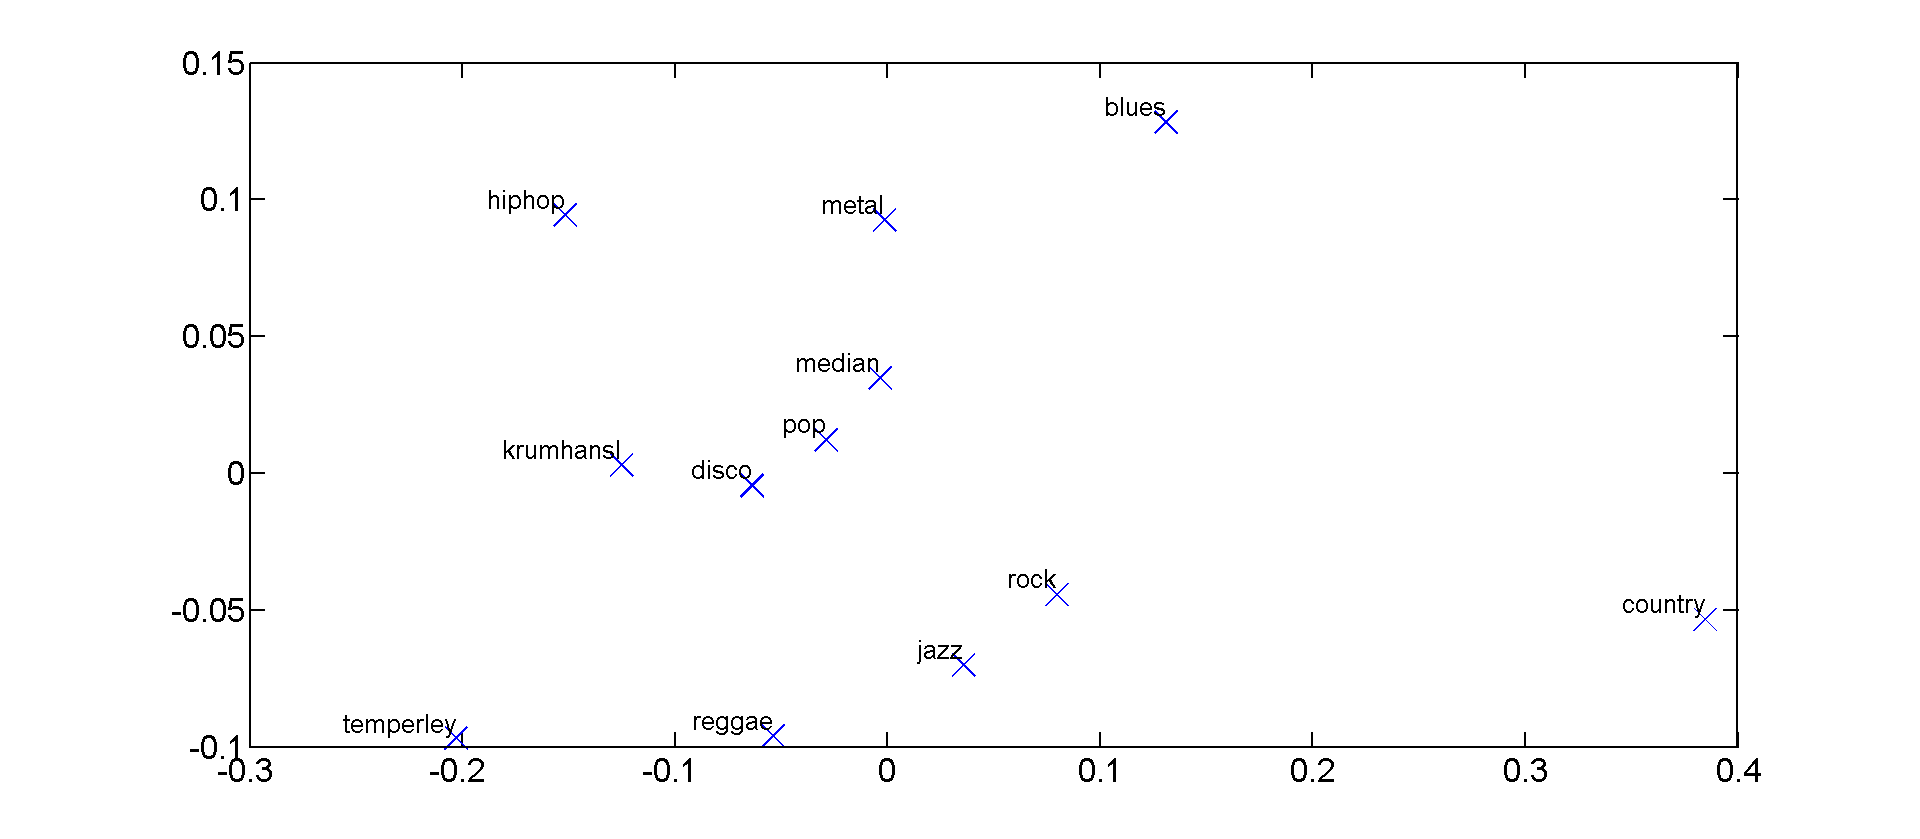
\includegraphics[scale=.2]{graph/MDS_min_colour}
	%\caption{MDS plots for Major and Minor profiles using L1 distance}
	%\label{fig:MDS}
%\end{figure}
%%



\begin{figure}\setcounter{figure}{1}
    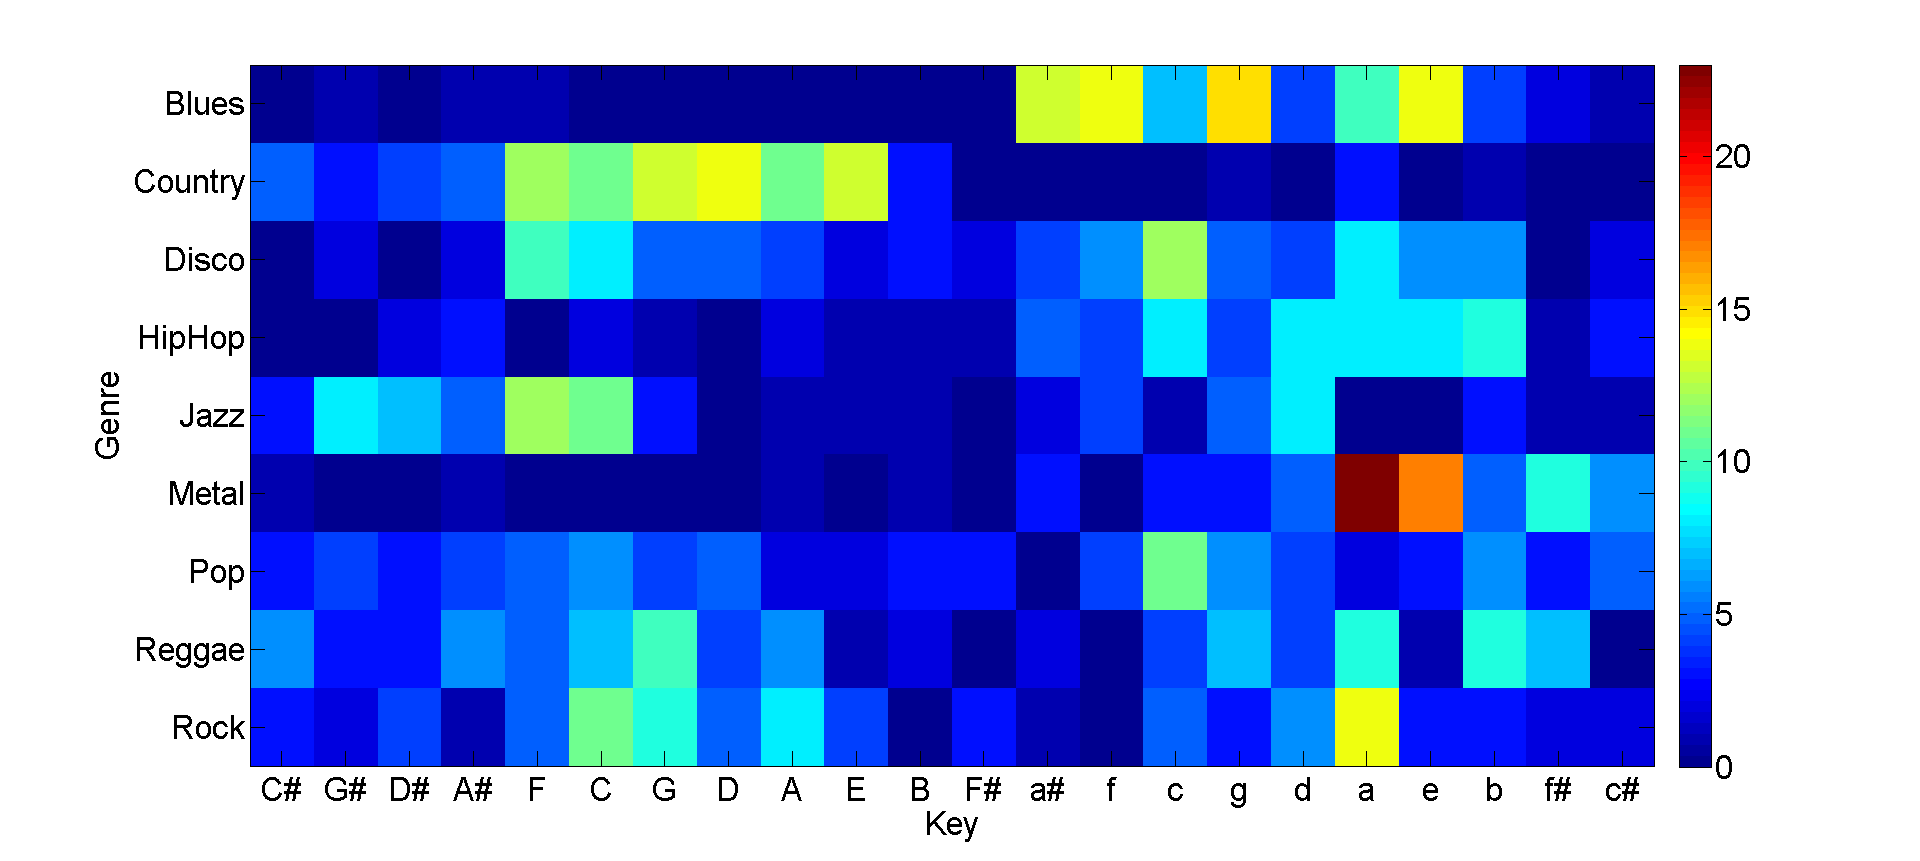
\includegraphics[scale=.2]{graph/key_distribution_colour_legend}
	\caption{Key distribution per genre}
	\label{fig:KeyDistributionPerGenre}
\end{figure}


\section{Classification}\label{sec:classification}
The distance results presented above indicate what genres are most similar and dissimilar (with respect to their key profiles). In order to drectly investigate the separability in terms of the key profiles, the extracted key profiles are used for the task of musical genre classification --  a well studied field in MIR \cite{fu_survey_2011}. The most widely used features in this area are timbre features such as Mel Frequency Cepstral Coefficients (MFCC). MFCC pick up on instrumental and timbral differences between genres, although they are not totally independent of harmonic and tonal properties \cite{li_genre_2011}.
A linear SVM classifier was trained using extraceted the key profiles. For comparison a linear SVM was also trained using $24$-dimensional timbre features vector comprising the mean and standard deviation of the first $12$ MFCCs. %The MFCC were calculated using a freely available MATLAB implementation.\footnote{\url{http://labrosa.ee.columbia.edu/matlab/rastamat/}}
We used libSVM  \cite{chang_libsvm:_2011} and picked the SVM parameters with a grid search and 5-fold cross validation on a separate stratified split of the data. The classification is carried out for the $9$ classes described above.

\begin{table}[H]
\centering
\resizebox{\columnwidth}{!}{%
        \begin{tabular}{|c||c|>{\columncolor[gray]{0.8}}c|c|c|>{\columncolor[gray]{0.8}}c|c|c|c|c||c|c|c|}
        \hline
        \textbf{Genre} &\ \textbf{B} & \ \textbf{C }& \ \textbf{D} & \ \textbf{H} & \ \textbf{J} & \ \textbf{M} & \ \textbf{P} & \ \textbf{Rg} & \ \textbf{R} & \ \textbf{Kr} & \ \textbf{Tp}  & \ \textbf{Mdn}\\
        \hline\hline
        \textbf{B}		 & 0    &0.29   &0.27   & 0.30   &0.27    &0.18    &0.22  &0.33    &0.28    &0.28    &0.39    &0.18\\
        \hline
\rowcolor[gray]{0.8}
        \textbf{C}  &0.29         &0    &0.46    &0.59   &0.36    &0.45    &0.43    &0.43    &0.36   &0.53    &0.53    &0.41\\
        \hline
        \textbf{D} 	&0.27    &0.46         &0    &0.17    &0.20    &0.16    &0.10    &0.15    &0.19    &0.14    &0.20    &0.12\\
        \hline
        \textbf{H} & 0.30    &0.59    &0.17         &0    &0.28    &0.21    &0.17    &0.23    &0.33    &0.17    &0.27    &0.18\\
        \hline
\rowcolor[gray]{0.8}
        \textbf{J} 		&0.27    &0.36    &0.20    &0.28         &0    &0.23    &0.16    &0.19    &0.16    &0.24    &0.27    &0.15\\
        \hline
        \textbf{M} 	& 0.18    &0.45    &0.16    &0.21    &0.23         &0    &0.13    &0.26    &0.20    &0.14    &0.31    &0.09\\
        \hline
        \textbf{P} 		&0.22    &0.43    &0.10    &0.17    &0.16    &0.13         &0    &0.15    &0.16    &0.13   &0.25    &0.05\\
        \hline
        \textbf{Rg} 	&0.33    &0.43    &0.15    &0.23    &0.19    &0.26    &0.15         &0    &0.19    &0.18    &0.23    &0.18\\
        \hline
        \textbf{R} 		&0.28   &0.36    &0.19    &0.33    &0.16    &0.20    &0.16    &0.19         &0    &0.25    &0.33    &0.15\\
        \hline\hline
				\textbf{Kr} 		&0.28    &0.53    &0.14    &0.17    &0.24    &0.18    &0.13    &0.18    &0.25         &0    &0.16    &0.16\\
				\hline
				\textbf{Tp} 		& 0.39    &0.53    &0.20    &0.27    &0.27    &0.31    &0.25    &0.23    &0.33    &0.16         &0    &0.28\\
				\hline
				\textbf{Mdn} 		&0.18    &0.41    &0.12    &0.18    &0.15    &0.09    &0.05    &0.18    &0.15    &0.16    &0.28         &0\\
				\hline
        \end{tabular}%
}
   
	\caption{Genre Distances for Minor tracks using L1-norm}
	\label{tab:GenreDistancesMinor}
\end{table}

\begin{table}[H]
\centering
\resizebox{\columnwidth}{!}{%
        \begin{tabular}{|c||>{\columncolor[gray]{0.8}}c|c|c|>{\columncolor[gray]{0.8}}c|c|>{\columncolor[gray]{0.8}}c|c|c|c||c|c|c|}
        \hline
        \textbf{Genre} & \textbf{B} & \ \textbf{C }& \ \textbf{D} & \ \textbf{H} & \ \textbf{J} & \ \textbf{M} & \ \textbf{P} & \ \textbf{Rg} & \ \textbf{R} & \ \textbf{Kr} & \ \textbf{Tp}  & \ \textbf{Mdn}\\
        \hline\hline
\rowcolor[gray]{0.8}
        \textbf{B}		 &0    &0.35    &0.40    &0.68    &0.44    &0.34    &0.35    &0.43    &0.31    &0.51    &0.59    &0.33\\
        \hline
        \textbf{C}  &0.35         &0    &0.27    &0.60    &0.32    &0.32    &0.17    &0.34    &0.20    &0.41    &0.47    &0.19\\
        \hline

        \textbf{D} 	&0.40    &0.27         &0    &0.33    &0.12    &0.21    &0.11    &0.12    &0.11    &0.15    &0.25    &0.09\\
        \hline
\rowcolor[gray]{0.8}
        \textbf{H} 	&0.68    &0.60    &0.33         &0    &0.27    &0.41    &0.42    &0.28    &0.43    &0.24    &0.29    &0.40\\
        \hline
        \textbf{J} 		&0.44    &0.32    &0.12    &0.27         &0    &0.25    &0.15    &0.17    &0.17    &0.12    &0.24    &0.13\\
        \hline
\rowcolor[gray]{0.8}
        \textbf{M} 	&0.34    &0.32   &0.21    &0.41    &0.25         &0    &0.20    &0.21    &0.16    &0.27    &0.41    &0.19\\
        \hline
        \textbf{P} 		&0.35    &0.17    &0.11    &0.42    &0.15    &0.20         &0    &0.19    &0.08    &0.23    &0.29    &0.05\\
        \hline
        \textbf{Rg} 	&0.43    &0.34    &0.12    &0.28    &0.17    &0.21    &0.19         &0    &0.17    &0.13    &0.23    &0.17\\
        \hline
        \textbf{R} 		&0.31    &0.20   &0.10    &0.43    &0.17    &0.16    &0.08    &0.17         &0    &0.23   &0.30    &0.06\\
        \hline\hline
				\textbf{Kr} 		&0.51    &0.41   &0.15    &0.24    &0.14    &0.27    &0.23    &0.13    &0.23         &0    &0.15    &0.21\\
				\hline
				\textbf{Tp}		&0.59   &0.47    &0.25    &0.29    &0.24    &0.41    &0.29    &0.23    &0.30    &0.15         &0    &0.28\\
				\hline
				\textbf{Mdn} 		&0.33    &0.19    &0.09    &0.40    &0.13    &0.19    &0.05    &0.17    &0.06    &0.21    &0.28         &0\\
				\hline
        \end{tabular}%
}
    
   
	\caption{Genre Distances for Major tracks using L1-norm}
	\label{tab:GenreDistancesMajor}
\end{table}

For the distance measure presented above, the extracted pitch chroma was shifted by the tonic from the ground truth (referred to as KP3 below). While such key profiles can be used to show similarity, they can not used in a general classification scenario as no key label will be available. Therefore, we also evaluated the following approaches to estimating a key-independent representation:
\begin{inparaenum}[(i)]
    \item   \textit{KP0: unshifted} ---
        the overall pitch chroma of each song is used as extracted;
    \item   \textit{KP1: transposition by max} ---
        the overall pitch chroma of each song is shifted by the index of the maximum of this pitch chroma. Detecting the index of the maximum can be interpreted as the simplest possible tonic estimation;
    \item   \textit{KP2: Fourier transform} ---
        the shift dependent on the tonic can be understood as the phase of the pitch chroma. The magnitude spectrum of the extracted pitch chroma is thus a phase-independent (and therefore tonic independent) representation; %Firstly, for a given pitch chroma vector the mean over all bins is calculated and is subtracted from each component. 
    \item   \textit{KP3: transposition by ground truth} ---
        the overall pitch chroma of each song is shifted by the tonic index annotated in the ground truth.
\end{inparaenum}
Three classification scenarios have been evaluated: 
\begin{inparaenum}[(i)]
    \item   only major keys, 
    \item   only minor keys, and 
    \item   the whole key-labeled data set without any differentiation between major and minor. 
 \end{inparaenum}   
All scenarios were carried out with the individual key profile features as well as with the combination of MFCCs and these features. The presented results are computed with 10-fold cross validation.
\subsection{Results and discussion}
Table~\ref{tab:accuracyPC} summarizes the results of the SVM classification for the different key profile computations and their performance when combined with the MFCCs. 

A minimum result is the output of a hypothetical classifier that simply predicts the majority class (ZeroR). The classification accuracy for this minimal classifier for our data set would be 26\% for Major, 20\% for Minor, and 13\% for the overall data set. The accuracy of a random pick is approximately 11\%. The results of Tzanetakis and Cook  reported, a 23\% classification accuracy  for the complete set with $10$ classes (i.e., including samples with ambiguous tonality) using a GMM 

%Zero-R classifier predicts 26\% accuracy for major profiles, 20\% for minor and approximately 11\% for random guessing.

\begin{table}[H]
\begin{center}
\resizebox{\columnwidth}{!}{%
    \begin{tabular}{|l|l|l|l|}
      \hline 
	\bf Feature & \bf Major & \bf Minor & \bf All\\
	\hline
	KP0 & 35.35 $\pm$ 2.53 & 37.90 $\pm$ 1.39 & 35.04 $\pm$ 1.97\\
	\hline
	KP1 & 37.24 $\pm$ 2.35 & 34.72 $\pm$ 2.21 & 35.91 $\pm$ 1.65\\
	\hline
	KP2 & 37.74 $\pm$ 2.29 & 36.36 $\pm$ 2.58 & 32.36 $\pm$ 2.08\\
	\hline
	KP3 & 40.33 $\pm$ 2.04 & 39.66 $\pm$ 3.33 & 33.83 $\pm$ 0.92\\
 	\hline\hline
	MFCC & 57.26 $\pm$ 1.50 & 64.33 $\pm$ 1.69 & 58.25 $\pm$ 2.55\\
	\hline
	KP0+MFCC & 59.17 $\pm$ 1.98 & 66.84 $\pm$ 2.57 &  62.44 $\pm$ 1.76\\
	\hline
	KP1+MFCC & 61.88 $\pm$ 1.34 & 64.27 $\pm$ 2.22  &  62.86 $\pm$ 1.73 \\
	\hline
	KP2+MFCC & 61.53  $\pm$ 1.65  & 62.08 $\pm$  2.49 &  61.48 $\pm$ 1.38 \\
 	\hline
	KP3+MFCC & 61.96 $\pm$ 1.42 & 67.37 $\pm$ 1.46& 63.10 $\pm$ 2.39\\
 	\hline

    \end{tabular}
    }
    \caption{Average classification accuracy and standard deviation over folds for different feature combinations.}
    \label{tab:accuracyPC}
  \end{center}
\end{table}

classifier with a set of simple pitch histogram features and a 47\% accuracy for 10 MFCCs \cite{tzanetakis_musical_2002}. These numbers may serve as a base-line comparison. 
%As with any classification task, the feature used to summarize tracks is an important concern. Previous work in this area has shown that timbral features, particularly Mel Frequency Spectrum Coefficients, are especially suited to the task of predicting genre. While MFCC are suited to picking up on instrumental and timbral difference between genres, some work has shown that they are not totally independent of harmonic or tonal information \cite{li_genre_2011}. Here we investigate the extent to which tonal information can be used to discern genres y examining the distributions of pitch chroma within each of 9 different genres. First we examine the overall distribution of keys for each genre. Next different methods for transposing pitch chroma to a key-independent representation are introduced and we look at the chroma distributions using chroma box plots, inter-genre distance and mulch-dimensional scaling. In the final section we test the degree to which the chroma distribution separate genres by performing classification with an SVM using chroma and combined chroma/MFCC features.


%To investigate this effect, we train and evaluate a Support Vector Machine using libSVM \cite{chang_libsvm:_2011}.
%The SVM hyper-parameters (C, \gamma) representing the margin and kernel widths were tuned using a grid-search and 5-fold cross validation on a separate stratified split of the data (I HAVE NO IDEA WHAT THAT MEANS). Best performance was achieved using a non-linear SVM with Radial Basis Function kernel.
%We investigated the following scenarios: (i) the whole key-labeled data set with no differentiation between major and minor and (ii) the major/minor subsets individually in order to control for the differences in major/minor distribution between keys. 
%10-fold cross validation  accuracy was calculated using the raw pitch chroma, max-shifted key profile, the Fourier pitch chroma and the key profile shifted according to the ground truth. We compare the results to a classifier based on a set of MFCC features as well as a combination of MFCC and key profile features. MFCC features were calculated according to REFXXX: WHAT COMPUTATION DID YOU USE?. The mean and standard deviation of $12$ MFCCs form a $24$-dimensional timbre feature vector. %as follows: for each block we compute 12 MFCC coefficients, then take the mean and standard deviation over the whole song. These features are then concatenated to form a 24 dimensional feature vector.

%Unsurprisingly, the 
MFCCs vastly outperformed the key profile features alone. Although not random, the overall classification performance given the key profiles is mediocre. While the key profiles provide genre-specific information, there are apparently still a lot of inter-genre similarities. The combined feature set results in a slight performance increase in overall accuracy of around 3-4\% indicating that the pitch chroma distributions contain some genre-relevant information not covered by the MFCCs. 

For the Major and Minor subsets, we can observe a slight performance increase for the shifted profiles (most notably the KP3 profile, shifted by the ground truth). That indicates that when combining Major and Minor keys in one data set, the tonic information is actually more important for classification than the mode. It also indicates that overall, the distances between Major and Minor profiles are larger than the distances between genre profiles. 

It should be noted that neither the shifting by ground truth data nor the split of the data set into Major and Minor modes represent a realistic classification scenario, since this data is not available (or could be only by estimating the key before classifying, adding an additional source of error to the analysis). 
Still, the objective of this analysis was to investigate the separability of tonic independent key profiles; we can at least observe some inter-genre separability.


%One fact revealed in this analysis is the relatively small performance increase observed by sorting the chroma, even when using the ground truth directly. By sorting the chroma any information on the genre given by the key has been removed (for example as a prior estimate based on the key distributions in each genre) which would, it is hoped, reveal any differences in the distributions. Splitting the data into major and minor results in slightly improved accuracy, however in this case we have added information by using the ground truth and realistically harmony estimation should be done automatically which would be an additional source of error. 

%Tables~\ref{tab:confMatMajPC} and \ref{tab:confMatMinPC} display the confusion matrices of the classification results with the KP3 features. The confusion matrices give more detailed insight into which genres are more separable than others. %, and also allow some insights on the classifier performance in the case of non-uniform class distributions.
%MAYBE INCLUDE A 'BASELINE' CLASSIFICATION BASED ONLY ON THE KEY (NOT THE PITCH CHROMA) HERE FOR COMPARISON???

%\begin{figure}[tb]
%    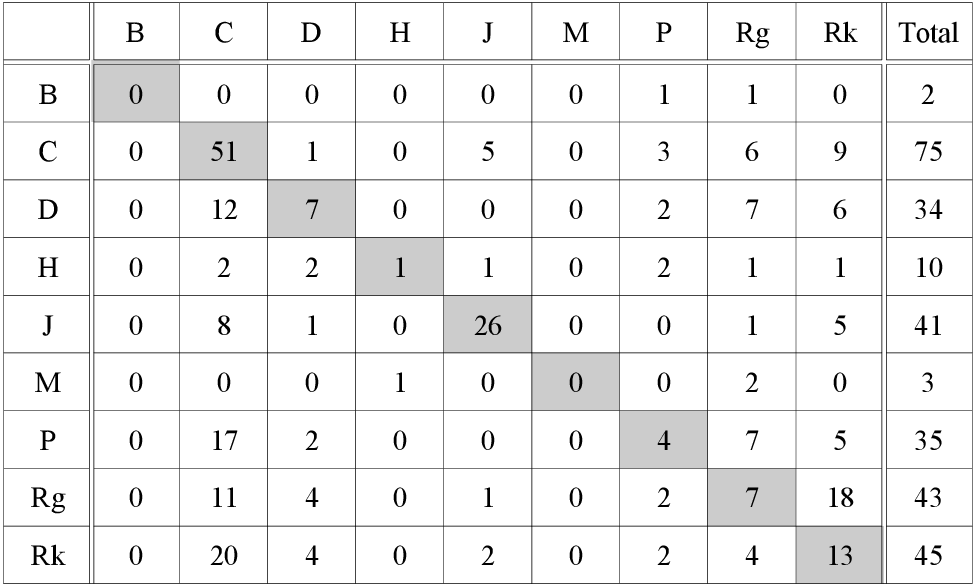
\includegraphics[scale=.4]{graph/confMatMajPC}
%	\caption{CONFUSION MATRIX 1, major}
%	\label{fig:confMatMajPC}
%\end{figure}

%\begin{itemize}
%    \item   table: profile-based classification worse than timbre classification
%    \item   table: ground truth shifting better than other features, except when combining modes
%    \item   table: FFT shift in the same range as Max shift
%    \item   table: unshifted not much worse than shifted
%    \item   major confusion matrix: many classifications into country, minor confusion matrix: many classifications into  metal --- why?
%\end{itemize}


%The confusion matrices let us observe a strong tendency for the classifier to choose the majority class. For Major, this is the class country and for Minor the classes metal and blues. 
%The genres with the highest classification  accuracies are country and jazz for Major and blues, hip-hop and metal for minor. 
%The results agree with the MDS plot in \secref{keyprof} in that the most distant genres in that plot seem to receive the highest classification accuracies. 
%Given the overall range of the classification results, however, a more detailed interpretation would be most likely more speculative than evidence-based.


\section{Conclusion}
We presented an analysis of key profiles for different genres and investigated inter-genre distances and separability using distance measures and classification. The results show that some genres may indeed have distinct key profiles, but overall, the similarities between key profiles seems to outweigh the genre differences. The classification results show modest improvements by using the shifted key profiles instead of the average pitch chroma, indicating the usefulness of the tonic-normalized pitch chroma. %These improvements, however, disappear when Major and Minor samples are not treated separately (which, in the case of classification, would be the normal case as the key is unknown). %Possible other reasons for the very slight accuracy improvements might be found in the data set (definition of genres, sample selection, size, other deficiencies), but in general we believe that the results make sense and are conceivable.
%
Overall, the results support the notion of using genre-independent profiles as inter-genre differences are small and in a similar range as inter-song differences between profiles. 

%\begin{table}[H]
%\begin{center}
%\resizebox{\columnwidth}{!}{%
%    \begin{tabular}{|l|l|l|l|l|l|l|l|l|l|l|}
%      \hline 
%  & \bf B &\bf C  &\bf D &\bf H &\bf J &\bf M &\bf P &\bf Rg &\bf Rk &\bf Total \\
%\hline
%\bf B & 0  & 0  & 0  &0  &0  &0  &1  &1  &0  &2  \\
%\hline
%\bf C & 0  & 51  &1 & 0 &5  &0  &3  &6  &9  &75\\
%\hline
%\bf D & 0  & 12  & 7 & 6 & 0 & 2 & 2 &7  &8  &44 \\
%\hline
%\bf H & 0  & 2  &2  &1  &1  &0  & 2 &1  &1  &10 \\
%\hline
%\bf J & 0  &8   & 1 &0  &26  &0  & 0 &1  & 5 & 41\\
%\hline
%\bf M  & 0  &0   &0  &1  &0  &0  &0  & 2 & 0 &3 \\
%\hline
%\bf P & 0  & 17   &2  &0  &0  &0  &4  &7  & 5 &35 \\
%\hline
%\bf Rg & 0  &11   &4  &0  &1  &0  &2  &7  &18  &43 \\
%\hline
%\bf Rk & 0  &20   &4  & 0 & 2 &0  &2  &4  & 13 & 45\\
%\hline
%\bf Total & 0  &121   &21  &2  &35  &0  &16  & 36 &57  & \\
%\hline
%    \end{tabular}
%    }
%    \caption{Confusion matrix, Major keys}
%    \label{tab:confMatMajPC}
%  \end{center}
%\end{table}
%\begin{itemize}
%    \item   some genres are separable, but overall the similarities between the key profiles outweigh the differences
%    \item   mention most similar and most separate genres
%    \item   not a proposal to use these profiles but to investigate whether there are genre dependent differences or not.
%\end{itemize}

%\begin{table}[H]%[!t]
%\begin{center}
%\resizebox{\columnwidth}{!}{%
%    \begin{tabular}{|l|l|l|l|l|l|l|l|l|l|l|}
%      \hline 
%  &\bf B &\bf C  &\bf D &\bf H &\bf J &\bf M &\bf P &\bf Rg &\bf Rk &\bf Total \\
%\hline
%\bf B &51  & 0  &1  &3  &  4&14  & 2 &0  &1  &76 \\
%\hline
%\bf C &2  &  0 & 0 &0  & 0 &1  &0  &1 &0  &4 \\
%\hline
%\bf D &1  &0   &14  &8  &0  & 12 &4  &3  &2  &44 \\
%\hline
%\bf H &30 &0   &2  &32  &0  & 13 &1  &4  &0  &55 \\
%\hline
%\bf J &12  & 0  & 1 &0  &8  &0  &0  &0  &0  &21 \\
%\hline
%\bf M  &14  &0   &4  &14  &0  &34  &3  & 1 & 1 &71 \\
%\hline
%\bf P &7  &0   &8  & 7 & 0 &15  &1  &1  &1  &40 \\
%\hline
%\bf Rg &2  &0   & 2 & 8 & 0 &9  &3  & 10 &1  &35 \\
%\hline
%\bf Rk & 13 &   0&  4&1  & 0 &7  & 1 & 5 &3  &34 \\
%\hline
%\bf Total & 132 & 0  & 36 & 73 &12  &105  & 15 &25  &9  & \\
%\hline
%    \end{tabular}
%    }
%    \caption{Confusion matrix, Minor keys}
%    \label{tab:confMatMinPC}
%  \end{center}
%\end{table}   

\bibliography{ChromaPaper}
\end{document}





% -----------------------------------------------
% Template for ISMIR 2014
% (based on earlier ISMIR templates)
% -----------------------------------------------
%
%\documentclass{article}
%\usepackage{ismir2014,amsmath,cite}
%\usepackage{graphicx}
%\usepackage{url}
%\usepackage{units}
%\usepackage{booktabs}
%\usepackage{dcolumn}
%\usepackage{colortbl}
%\usepackage{microtype}
%\usepackage{float}
%
%% Title.
%% ------
%\title{}
%
%% Single address
%% To use with only one author or several with the same address
%% ---------------
%%\oneauthor
%% {Names should be omitted for double-blind reviewing}
%% {Affiliations should be omitted for double-blind reviewing}
%
%% Two addresses
%% --------------
%%\twoauthors
%%  {First author} {School \\ Department}
%%  {Second author} {Company \\ Address}
%
%% Three addresses
%% --------------
%\threeauthors
  %{First author} {Affiliation1 \\ {\tt author1@ismir.edu}}
  %{Second author} {\bf Retain these fake authors in\\\bf submission to preserve the formatting}
  %{Third author} {Affiliation3 \\ {\tt author3@ismir.edu}}
%
%% Four addresses
%% --------------
%%\fourauthors
%%  {First author} {Affiliation1 \\ {\tt author1@ismir.edu}}
%%  {Second author}{Affiliation2 \\ {\tt author2@ismir.edu}}
%%  {Third author} {Affiliation3 \\ {\tt author3@ismir.edu}}
%%  {Fourth author} {Affiliation4 \\ {\tt author4@ismir.edu}}
%
%\begin{document}
%%
%\maketitle
%%
%\begin{abstract}
%\end{abstract}
%%
%
%
%\end{document}
